\documentclass[../main.tex]{subfiles}
\begin{document}
\chapter{Expanded envelopes}\label{chapter4}
For the same neutron star of mass $M=1.4 \Msun$ and radius $R=12$ km, we now search for solutions to the equations of structure with $u=0$. The resulting profiles will represent expanded static envelopes where hydrostatic balance is sustained by the luminosity. As explained in the introduction, the local luminosity is a function of redshift (Eq.~\ref{eq:Linf}), with the luminosity at infinity $L
^\infty$ being a constant of each model.  The other free parameter which will determine the model is the photospheric radius $r\ph$, which we will define in a slightly different way than in the wind models. The boundary condition at the surface will be the same as in the wind models, so that we will be able to link burning layer conditions to either regime. 

As in the wind case, we integrate the equations of structure derived in Chapter \ref{chapter2}. However, it is worth mentioning that in the static ($u=0$) case, these equations can be re-written in a way that is perhaps more intuitive to understand. Indeed, we can write
\begin{align}
    \frac{dP}{dr}&=-\frac{GM\rho}{r^2\zeta^2}\left[1+\left(4-\frac{3}{2}\beta_i-\frac{3f-4}{f-1}\beta_e\right)\frac{P}{\rho c^2}\right] \label{eq:env_dPdr}\\
    \frac{d\rho}{dr}&=\frac{\rho}{P}\frac{dP}{dr}\frac{\left[1-(4-3\beta_i-(4-\alpha_1)\beta_e)\nabla_\text{rad}\right]}{\beta_i+\beta_e(\alpha_1+\alpha_2f)} \label{eq:env_drhodr}\\
    \frac{dT}{dr}&=\frac{T}{\rho}\frac{dP}{dr}\nabla_\text{rad} \label{eq:env_dTdr}\,,
\end{align}
where
\begin{align}
    \label{eq:delrade}
    \nabla_\text{rad}&=\left[\frac{\zeta\kappa L_\infty}{16\pi GMc(1-\beta_i-\beta_e)}+\frac{P}{\rho c^2}\right] \nonumber\\
    &\times \left[1+\left(4-\frac{3}{2}\beta_i-\left(\frac{3f-4}{f-1}\right)\beta_e\right)\frac{P}{\rho c^2}\right]^{-1}
\end{align}
is the radiative gradient. In the non-degenerate limit, these equations are the same as those written by \citet{Paczynski1986a} for an ideal gas plus radiation EOS. Eq.~\ref{eq:env_dPdr} is just the statement of hydrostatic equilibrium, with the proper GR and degenerate EOS corrections, Eq.~\eqref{eq:env_drhodr} can be directly derived from Eq.~\eqref{eq:env_dPdr}, and Eq.~\ref{eq:env_dTdr} is another way to write the photon diffusion equation~\eqref{eq:photondiffusion}.  Writing these equations in terms of the radiative gradient is relevant, because in order for heat to be transported by radiation rather than convection, the following condition must be respected at every point:
\begin{equation}\label{eq:nabla_condition}
    \nabla_\text{rad}<\nabla_\text{ad}\,,
\end{equation}
where
\begin{equation}
    \nabla_\text{ad}\equiv\left(\frac{\partial\ln T}{\partial\ln P}\right)_s
\end{equation}
is the adiabatic gradient. The ``$s$'' subscript indicates a derivative with constant entropy. If $\nabla_\text{ad}$ becomes the smaller gradient, then the envelopes will become convective \citep{Paczynski1986a}. We are ignoring convection in our model, so we must verify that Eq.~\eqref{eq:nabla_condition} is true at every point in the envelopes.

We present present our numerical method for calculating envelope models in \S\ref{sec:env_numerical_integration} and analyze the results in \S\ref{sec:env_results}. In \S\ref{sec:compact_envelopes}, we discuss the errors that can be made on the neutron star radius if one of these envelopes is present at touchdown.


\section{Numerical integration  and boundary conditions}\label{sec:env_numerical_integration}
%To calculate wind solutions, we use an approach similar to \citet{Paczynski1986b} in that we start at the critical point and integrate outward to the photosphere and inward to the star's surface, checking if the boundary conditions are met at both ends and changing the free parameters until they are. We apply the same procedure for every mass-loss rate $\Mdot$ in order to have a single wind model for each value.  All integrations are done using fully implicit ODE solvers provided by the \textit{SciPy} numerical package \citep{SciPy}.\\

%The critical point is first found based on a trial value for its temperature $T_c$ by finding the unique root to Eq.~\eqref{eq:regularity_constraint}. This also indirectly sets the free parameter $L_b$ through the energy equation \eqref{eq:Edot} by initializing the temperature profile. Not all values of $r_c$ are acceptable. For instance, if $T_c$ is too high, the critical point can be located at $r<R$, under the surface of the star, such that the wind would start off supersonic at the base - we do not accept solutions of this kind.\\

%We then integrate equations \eqref{eq:dTdr} and \eqref{eq:dphidr} for $T$ and $\Phi$, with initial va

Similar to the method used by \citet{Paczynski1986a}, we look for envelope solutions for every value of $r\ph$ by setting trial values for $L\ph$, then integrate inwards to see how far the envelope base is from the neutron star surface, then adjust $L\ph$ accordingly. We explain the details of this process and the method for constructing the final solution in what follows. 

As explained in Chapter \ref{chapter1}, envelopes are sustained by a luminosity that is only slightly sub-critical everywhere. We define the luminosity parameter
\begin{equation}\label{eq:env_qparam}
    q\equiv 1-\frac{L}{\Lcr}\,,
\end{equation}
which we expect to be very close to zero everywhere, but always positive. To find the envelope model for a given $r\ph$, we begin by adopting a trial value for $\log_{10}q\ph$, which we know to be between $-4$ and $-3.5$ from the work of \citet{Paczynski1986a}. Then, we initilalize the variables $\rho$ and $T$ based on the outer boundary condition which defines the photosphere. For temperature, we assert that $T\ph=T_\text{eff}$, just like in the wind case. This implies
\begin{equation}\label{eq:env_Tph}
    T\ph^4=\frac{L\ph}{4\pi r\ph^2\sigma}=\frac{\Lcr(1-q\ph)}{4\pi r\ph^2\sigma}\,,
\end{equation}
where $\Lcr$ itself depends on the temperature via the opacity $\kappa(T)$ (Eq.~\ref{eq:kappa}). Therefore, we re-write Eq.~\eqref{eq:env_Tph},
\begin{equation}
    0=\kappa(T\ph)T\ph^4-\frac{GMc(1-q\ph)}{r\ph^2\sigma}\left(1-\frac{r_s}{r\ph}\right)^{-1/2}\,,
\end{equation}
such that $T\ph$ can be found with a simple one-dimensional root-finding algorithm. The luminosity at infinity can now be found with
\begin{equation}\label{eq:env_Linf}
    L^\infty=\Ledd \frac{\kappa_0}{\kappa(T\ph)}(1-q\ph)\left(1-\frac{r_s}{r\ph}\right)^{1/2}
\end{equation}

To find the initial density, we start by making use of the fact that $u=du/dr=0$ to re-write the initial momentum equation,
\begin{equation}
    \omega_g\frac{d\ln\Psi}{dr} + P_g' - \frac{1}{c\Psi}\rho\kappa F = 0\,,
\end{equation}
as
\begin{equation}
    \frac{dP_g}{dr}=-\frac{g\rho}{\zeta}\left(1+\frac{5}{2}\frac{kT}{\mu m_pc^2}-\frac{L}{\Lcr}\right)\,,
\end{equation}
where we used the ideal gas EOS for $\omega_g$, since degenerate corrections will not matter near the photosphere. In any case, we can neglect the gas term since $kT/m_p\ll c^2$. Further, we can use the differential form of the definition for the true optical depth (Eq.~\ref{eq:trueopticaldepth}),
\begin{equation}
    d\tau=-\rho\kappa\frac{dr}{\zeta}\,,
\end{equation}
in order to finally rewrite the pressure gradient as \footnote{Do note that Eq.~\eqref{eq:dPg_dtau} is only valid under the approximations of hydrostatic equilibrium and negligible gas pressure.}
\begin{equation}\label{eq:dPg_dtau}
    \frac{dP_g}{d\tau}=\frac{gq}{\kappa} \,.
\end{equation}
We can integrate this equation from infinity ($\tau=0$) until the photosphere. This time, we can set a boundary value for the true optical depth, instead of $\tau^*$ like in the wind case. For stellar grey atmospheres, the value $\tau=2/3$ defines the photosphere when the Eddington approximation\footnote{Radiation pressure equals a third of the radiation energy density. We already made use of this approximation in Chapter \ref{chapter2}.} is taken \citep{Mihalas1978}. Assuming zero gas pressure at infinity and that $L$,$\Lcr$ and $\kappa$ are approximately constant everywhere beyond $\tau=2/3$, we get the condition for the density at the photosphere:
\begin{equation}\label{eq:env_rhoph}
    \rho\ph=\frac{2}{3}\frac{gq}{\kappa(T\ph)}\frac{\mu m_p}{kT\ph}\,.
\end{equation}
This boundary condition given by equations \eqref{eq:env_Tph} and \eqref{eq:env_rhoph} was also used by \citet{Paczynski1986a}. 

We integrate $T$ and $\rho$ from these initial values using equations \eqref{eq:dTdr} and \eqref{eq:drhodr}, and stop once we hit the base radius $r_b=r(y=P/g=10^8)$. The inner boundary condition for matching to the surface,
\begin{equation}\label{eq:env_innerbc}
    r_b=R\,,
\end{equation}
is the same as in the wind case. Ideally, we would simply iterate on $q\ph$ until Eq.~\eqref{eq:env_innerbc} is satisfied. However, we found that this was not generally possible, as it would require us to increase the number of digits of $q\ph$ and decrease the numerical routine tolerances beyond reasonable. In other words, there does exist an exact value of $q\ph$ that results in an envelope which follows the inner boundary condition Eq.~\eqref{eq:env_innerbc}, but calculating this envelope from a simple shooting method is not feasible numerically. Instead, we proceed with a stepwise bisection-like method. First, we find two nearby values of $q\ph$  for which the inwards integrations land on either side of the stellar radius, i.e. one has $r_b<R$ and the other has $r_b>R$. This way, we know the ``true'' value of $q\ph$ to be in between these two values. Then, we identify the first point of divergence in the integration, i.e. where the values of $T$ or $\rho$ of the two envelopes differ by more than the chosen relative tolerance of $10
^{-4}$. At this point, we interpolate the values for the two variables (take the middle value) to initialize a new envelope, which is bound by the initial two envelopes in both $\rho$ and $T$. We look at which side of $R$ this new envelope lands, and discard the initial envelope which lands on that same side. We then repeat the interpolation procedure at the next point of divergence, and so on until we have a solution which satisfies the boundary condition. Fig.~\ref{fig:env_bisection_demo} shows a visual demonstration of our method. 

After having constructed an envelope, we verified that we had truly found a solution to the equations of structure by interpolating a polynomial and comparing its derivatives at every $r$ to the ones prescribed by equations \eqref{eq:dTdr} and \eqref{eq:drhodr}.

\begin{figure}[htb!]
    \centering
    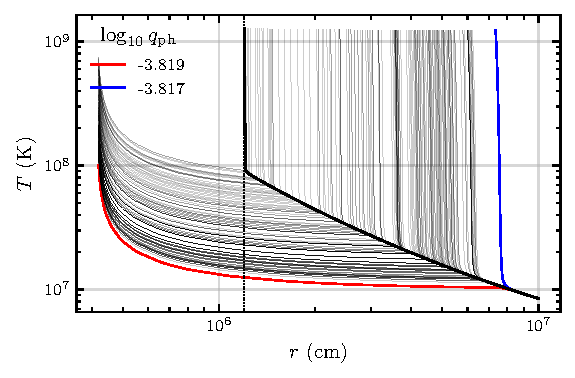
\includegraphics{figures/env_bisection_demo.pdf}
    \caption[Demonstration of the numerical method for envelopes]{Method for finding envelope solutions. Shown is a demonstration of the $r\ph=100$ km envelope. The blue and red lines are the two initial solutions, the thick black line is the final solution. The thin black lines are the intermediate solutions which start at every point of divergence in the inwards integration. The dashed vertical line marks the $r=R$ line. See text for more details.}
    \label{fig:env_bisection_demo}
\end{figure}


% \section{Results}\label{sec:env_results}
\section{Dependence of the envelope models on $r\ph$}\label{sec:env_results}
We calculated envelope models with the method described in the previous sections for very small photospheric radii just above the neutron star radius, all the way to very large values in the hundreds to one thousand kilometres. Fig.~\ref{fig:env_profiles} shows radial profiles of the temperature, density, and luminosity parameter $q$ for eight different envelope models. Just like in the wind case, most the the mass is stored in a compact region of only a few kilometres above the surface. After a drop in temperature and density of several orders of magnitude, the envelope transitions to an extended region which is still in hydrostatic equilibrium and can span hundreds of km. The bottom panel of Fig.~\ref{fig:env_profiles} confirms the statement made in section \ref{section:basic_theory} that $L\lesssim \Lcr$ at every $r$. This allows for a significant reduction of the effective gravity, allowing large expansion, while preventing outflows, thus maintaining equilibrium. 

Figure \ref{fig:env_rho_T} shows the temperature profiles as a function of density. All envelopes transition to the same radiation-dominated regime at low density. As was noted by \citet{Paczynski1986a}, this final state is independent of the base temperature. The envelopes are gas pressure dominated at the base, but they are too hot to be dominated by degenerate electrons. It is interesting to note that even with sub-Eddington luminosities, bursts can easily generate large enough temperatures to lift all degeneracies, at least at the depths with which we are concerned. It is easy to see that the degenerate regime could be reached by extending the curves in Fig.~\ref{fig:env_rho_T} to larger densities. 

As was mentioned at the beginning of this chapter, we need to make sure that these envelopes are not convective, by verifying that $\nabla_\text{rad}<\nabla_\text{ad}$ everywhere. Since we found that degenerate electron corrections were not important, we can take the ideal gas plus radiation equation of state for the adiabatic gradient, for which the expression

\begin{figure}[H]
    \centering
    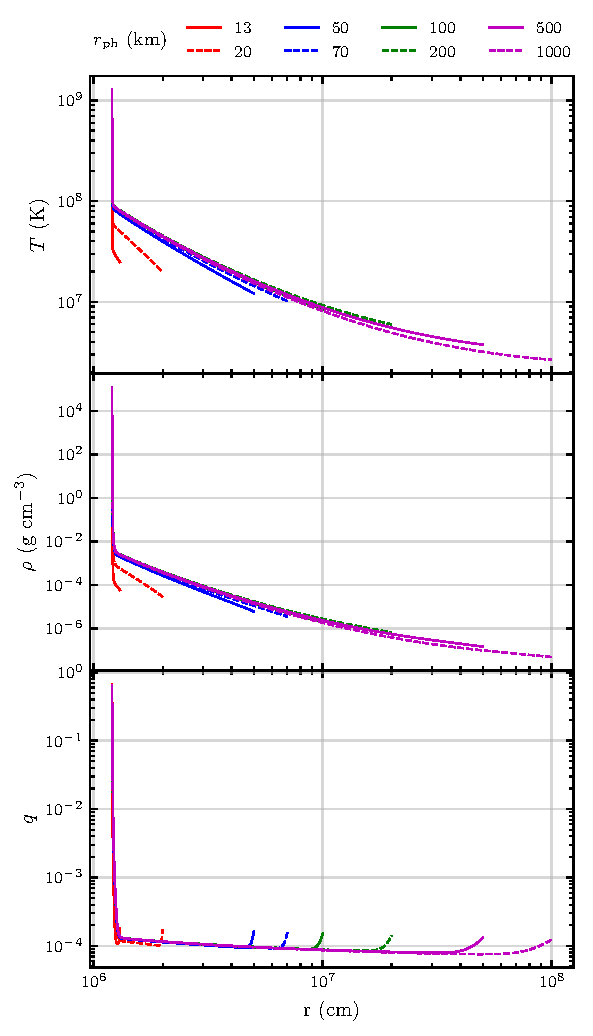
\includegraphics{figures/env_profiles.pdf}
    \caption[Envelope radial profiles]{Envelopes profiles from the base $r_b$ to the photosphere $r\ph$. Top to bottom: temperature, density, luminosity parameter $q$ (Eq.~\ref{eq:env_qparam})}
    \label{fig:env_profiles}
\end{figure}

\begin{figure}[H]
    \centering
    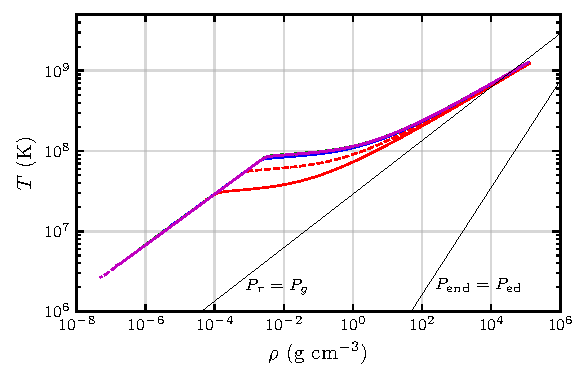
\includegraphics{figures/env_rho_T.pdf}
    \caption[Envelope temperature-density profiles]{Temperature-density profiles for the envelope. The colors refer to the same legend as Fig.~\ref{fig:env_profiles}. The black lines are explained in the caption of Fig.~\ref{fig:wind_rho_T}.}
    \label{fig:env_rho_T}
\end{figure}

\begin{equation}\label{eq:del_ad}
    \nabla_\text{ad}=\frac{8-6\beta}{32-24\beta-3\beta^2}
\end{equation}
is given in \citet{HansenKawaler1994}. Fig.~\ref{fig:env_del} demonstrates that our models are indeed radiative everywhere. However, it does appear that the extended regions of the envelopes are right on the verge of becoming convective, as the radiative gradient is only very slightly smaller than the adiabatic gradient. It could be relevant that the profiles of $1-\nabla_\text{rad}/\nabla_\text{ad}$ are similar to those of $q$, meaning the critical luminosity could be related to the onset of convection. There have been studies in the past of the relation between $L$, $\Lcr$ and radiative and convective regimes in stellar interiors (e.g. \citet{Joss1973}). The X-ray burst scenario is different in many ways to stellar interiors; in particular, we know from the work of \citet{Paczynski1986a} that general relativistic corrections to the critical luminosity are important for allowing very extended solutions. This warrants more investigation into the stability of our radiative envelope solutions, but is beyond the scope of this work. 

\begin{figure}[htb!]
    \centering
    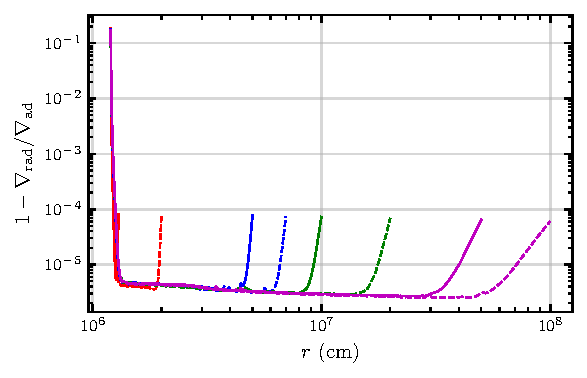
\includegraphics{figures/env_del.pdf}
    \caption[Envelope radiative to adiabatic gradient ratios]{Ratio of radiative gradient (Eq.~\ref{eq:delrade}) to adiabatic gradient (Eq.~\ref{eq:del_ad}).}
    \label{fig:env_del}
\end{figure}

Lastly, we discuss our results for the main observable, $L^\infty$ for these envelope models, which is shown as a function of $r\ph$ in Fig.~\ref{fig:env_rphot}. Whereas \citet{Paczynski1986a} found that their envelope models had $0.7<L^\infty/\Ledd<1$, our models have $0.85<L^\infty/\Ledd\lesssim 1.02$. Indeed, the most extended photospheres are in fact slightly super-Eddington, even if no wind is driven, though only by a few percent. This can be explained by looking at Eq.~\eqref{eq:env_Linf}, which shows that $L
^\infty/\Ledd$ is determined by three factors of order unity: the opacity ratio, luminosity parameter and redshift, all taken at the photosphere. \citet{Paczynski1986a} incorrectly took the first two factors as being equal to unity, saying that $\kappa\approx\kappa_0$ and $L\approx\Lcr$ at the photosphere, such that the redshift is the only parameter which determines $L^\infty$. These are, of course, sensible approximations in a general sense. However, in the context of Eq.~\eqref{eq:env_Linf}, they result in missing some subtlety. For small $r\ph$, the temperature is large enough (see Fig.~\ref{fig:env_profiles}) that $\kappa(T\ph)$ is significantly smaller than $\kappa_0$ -- this explains our lower bound of 0.85 on $L
^\infty/\Ledd$, instead of Paczynski and Anderson's 0.7. For large $r\ph$, the redshift term is very small, and so is $1-q\ph$, as shown by the blue curve in Fig.~\ref{fig:env_rphot}. While $T\ph$ is smaller than in the small $r\ph$ models, it is still large enough that the opacity ratio can ``win'' over the other two, resulting in super-Eddington luminosities. These are important details as they change our interpretation of the observations. To our knowledge, the fact that super-Eddington luminosities can lead to static, non-outflowing, envelopes\footnote{We have only shown that static envelopes with slightly super-Eddington luminosities and very large photospheres are possible in theory, at least under the set of approximations (spherically symmetric, optically thick) that we made. Whether or not these can actually be formed during Type I X-ray bursts is a separate question, which we will discuss in the next chapter.} has not been discussed in the literature before. %However, the luminosity is only in excess over Eddington by less than ${\sim}2$\%, so this fact likely d

\begin{figure}[htb!]
    \centering
    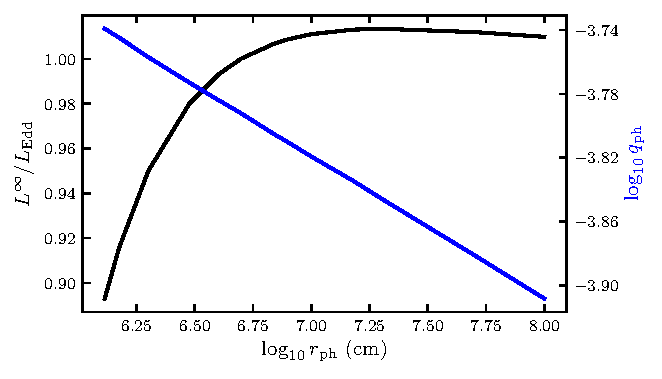
\includegraphics{figures/env_rphot.pdf}
    \caption[Envelope luminosities]{Luminosity parameters for all envelope models labelled by $r\ph$. Left axis, black line: luminosity at infinity, Eddington normalized. Right axis, blue line: luminosity parameter $q$ at the photosphere.}
    \label{fig:env_rphot}
\end{figure}

\section{Compact envelopes and touchdown radius}\label{sec:compact_envelopes}

We discussed in Chapter \ref{chapter1} the common technique of finding the neutron star radius based on the touchdown radius, i.e. the blackbody radius when the temperature peaks and the photosphere presumably touches back down to the surface following the PRE phase of the burst. But if the luminosity at the touchdown point is still near-Eddington, we have shown in this chapter that an expanded envelope could be present, which means that the photospheric (touchdown) radius is not the neutron star radius. We investigate in this section how important this error might be based on the observed parameters. To do this, we have extended our calculation of envelopes to very compact ones with photospheres less than 1 km above the neutron star surface.

The top panel of Fig.~\ref{fig:env_touchdown} shows that the range of luminosities that would cause a significant difference between the touchdown and neutron star radius (say more than 100 m) is quite narrow, from ${\sim}0.85\Ledd$ to $\gtrsim\Ledd$, but not inconceivable. Notice also that this problem only appears when factoring in general relativity, as Newtonian envelopes can only be very compact. In the bottom panel, if we look at $T_\text{eff}$, the effective temperature of the envelope (redshifted to infinity with $T^\infty=\zeta T$), we see that the peak of the temperature curve is very flat along $r\ph$. This means there is automatically uncertainty in the touchdown radius when inferring it from the temperature. For example, if the measured peak temperature is of $1.8\pm 0.1$ keV (an uncertainty of 5\%, which is generous if we look back to the errorbars in Fig.~\ref{fig:keek2018_fig3}), then Fig.~\ref{fig:env_touchdown} shows that the photospheric radius could be anywhere from just a few tens of meters to kilometres above the stellar surface. These results should motivate a more careful examination of the neutron star radii determined using the touchdown point.



\begin{figure}
    \centering
    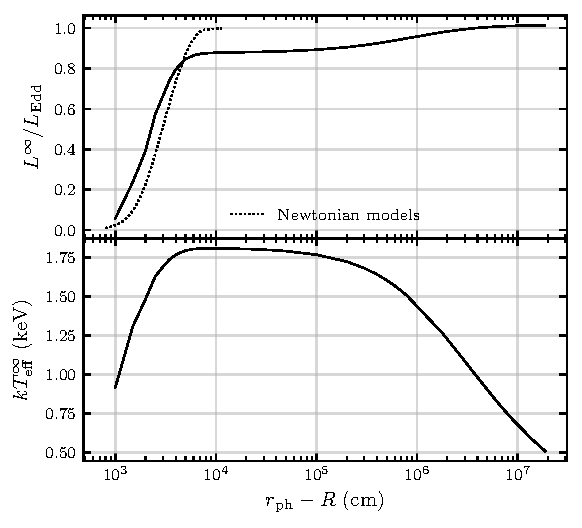
\includegraphics{figures/env_touchdown.pdf}
    \caption[Touchdown radius based on the observables]{Difference between the photospheric (touchdown) radius based on the luminosity (\textit{top}) and observed effective temperature (\textit{bottom}). The dotted line in the top panel represents Newtonian atmospheres, for which we derive an analytical formula in Appendix \ref{appendix_newtonian}.}
    \label{fig:env_touchdown}
\end{figure}


% example like if you measure kT with 5% uncertainty, according to the curve it's potentially 1km error.

\biblio
\end{document}
